\documentclass[journal, a4paper]{IEEEtran}

\usepackage[utf8x]{inputenc}
\usepackage[francais]{babel}

\usepackage{listings}

\usepackage{fancyvrb}

% some very useful LaTeX packages include:

%\usepackage{cite}      % Written by Donald Arseneau
                        % V1.6 and later of IEEEtran pre-defines the format
                        % of the cite.sty package \cite{} output to follow
                        % that of IEEE. Loading the cite package will
                        % result in citation numbers being automatically
                        % sorted and properly "ranged". i.e.,
                        % [1], [9], [2], [7], [5], [6]
                        % (without using cite.sty)
                        % will become:
                        % [1], [2], [5]--[7], [9] (using cite.sty)
                        % cite.sty's \cite will automatically add leading
                        % space, if needed. Use cite.sty's noadjust option
                        % (cite.sty V3.8 and later) if you want to turn this
                        % off. cite.sty is already installed on most LaTeX
                        % systems. The latest version can be obtained at:
                        % http://www.ctan.org/tex-archive/macros/latex/contrib/supported/cite/

\usepackage{graphicx}   % Written by David Carlisle and Sebastian Rahtz
                        % Required if you want graphics, photos, etc.
                        % graphicx.sty is already installed on most LaTeX
                        % systems. The latest version and documentation can
                        % be obtained at:
                        % http://www.ctan.org/tex-archive/macros/latex/required/graphics/
                        % Another good source of documentation is "Using
                        % Imported Graphics in LaTeX2e" by Keith Reckdahl
                        % which can be found as esplatex.ps and epslatex.pdf
                        % at: http://www.ctan.org/tex-archive/info/

%\usepackage{psfrag}    % Written by Craig Barratt, Michael C. Grant,
                        % and David Carlisle
                        % This package allows you to substitute LaTeX
                        % commands for text in imported EPS graphic files.
                        % In this way, LaTeX symbols can be placed into
                        % graphics that have been generated by other
                        % applications. You must use latex->dvips->ps2pdf
                        % workflow (not direct pdf output from pdflatex) if
                        % you wish to use this capability because it works
                        % via some PostScript tricks. Alternatively, the
                        % graphics could be processed as separate files via
                        % psfrag and dvips, then converted to PDF for
                        % inclusion in the main file which uses pdflatex.
                        % Docs are in "The PSfrag System" by Michael C. Grant
                        % and David Carlisle. There is also some information
                        % about using psfrag in "Using Imported Graphics in
                        % LaTeX2e" by Keith Reckdahl which documents the
                        % graphicx package (see above). The psfrag package
                        % and documentation can be obtained at:
                        % http://www.ctan.org/tex-archive/macros/latex/contrib/supported/psfrag/

%\usepackage{subfigure} % Written by Steven Douglas Cochran
                        % This package makes it easy to put subfigures
                        % in your figures. i.e., "figure 1a and 1b"
                        % Docs are in "Using Imported Graphics in LaTeX2e"
                        % by Keith Reckdahl which also documents the graphicx
                        % package (see above). subfigure.sty is already
                        % installed on most LaTeX systems. The latest version
                        % and documentation can be obtained at:
                        % http://www.ctan.org/tex-archive/macros/latex/contrib/supported/subfigure/

\usepackage{url}        % Written by Donald Arseneau
                        % Provides better support for handling and breaking
                        % URLs. url.sty is already installed on most LaTeX
                        % systems. The latest version can be obtained at:
                        % http://www.ctan.org/tex-archive/macros/latex/contrib/other/misc/
                        % Read the url.sty source comments for usage information.

%\usepackage{stfloats}  % Written by Sigitas Tolusis
                        % Gives LaTeX2e the ability to do double column
                        % floats at the bottom of the page as well as the top.
                        % (e.g., "\begin{figure*}[!b]" is not normally
                        % possible in LaTeX2e). This is an invasive package
                        % which rewrites many portions of the LaTeX2e output
                        % routines. It may not work with other packages that
                        % modify the LaTeX2e output routine and/or with other
                        % versions of LaTeX. The latest version and
                        % documentation can be obtained at:
                        % http://www.ctan.org/tex-archive/macros/latex/contrib/supported/sttools/
                        % Documentation is contained in the stfloats.sty
                        % comments as well as in the presfull.pdf file.
                        % Do not use the stfloats baselinefloat ability as
                        % IEEE does not allow \baselineskip to stretch.
                        % Authors submitting work to the IEEE should note
                        % that IEEE rarely uses double column equations and
                        % that authors should try to avoid such use.
                        % Do not be tempted to use the cuted.sty or
                        % midfloat.sty package (by the same author) as IEEE
                        % does not format its papers in such ways.

\usepackage{amsmath}    % From the American Mathematical Society
                        % A popular package that provides many helpful commands
                        % for dealing with mathematics. Note that the AMSmath
                        % package sets \interdisplaylinepenalty to 10000 thus
                        % preventing page breaks from occurring within multiline
                        % equations. Use:
%\interdisplaylinepenalty=2500
                        % after loading amsmath to restore such page breaks
                        % as IEEEtran.cls normally does. amsmath.sty is already
                        % installed on most LaTeX systems. The latest version
                        % and documentation can be obtained at:
                        % http://www.ctan.org/tex-archive/macros/latex/required/amslatex/math/



% Other popular packages for formatting tables and equations include:

%\usepackage{array}
% Frank Mittelbach's and David Carlisle's array.sty which improves the
% LaTeX2e array and tabular environments to provide better appearances and
% additional user controls. array.sty is already installed on most systems.
% The latest version and documentation can be obtained at:
% http://www.ctan.org/tex-archive/macros/latex/required/tools/

% V1.6 of IEEEtran contains the IEEEeqnarray family of commands that can
% be used to generate multiline equations as well as matrices, tables, etc.

% Also of notable interest:
% Scott Pakin's eqparbox package for creating (automatically sized) equal
% width boxes. Available:
% http://www.ctan.org/tex-archive/macros/latex/contrib/supported/eqparbox/

% *** Do not adjust lengths that control margins, column widths, etc. ***
% *** Do not use packages that alter fonts (such as pslatex).         ***
% There should be no need to do such things with IEEEtran.cls V1.6 and later.


% Your document starts here!
\begin{document}

% Define document title and author
	\title{Sécurité des réseaux}
	\author{Alexandre Kervadec
	\thanks{Professeur : A.Guermouche}}
	\markboth{Université de Bordeaux - Master 1 Informatique}{}
	\maketitle

% Write abstract here
\begin{abstract}
	Notes du cours de sécurité des réseaux de A.Guermouche
\end{abstract}

% Each section begins with a \section{title} command
\section{Les attaques}
	% \PARstart{}{} creates a tall first letter for this first paragraph
	\PARstart{O}{n} peut différencier une attaque d'une intrusion. Une attaque correspond à toute action compromettant la sécurité des informations. Une intrusion est la prise de contrôle partielle ou totale d'un système distant.
	
	\subsection{Description d'une attaque}
	
		\begin{itemize}
			\item \textbf{Recherche d'informations :} réseau, serveurs, routeurs, ...
			\item \textbf{Recherche de vulnérabilités :} OS, serveurs applicatifs, ...
			\item \textbf{Tentative d'exploitation des vulnérabilités :} à distance puis localement
			\item \textbf{Installation de backdoor}
			\item \textbf{Installation de sniffer}
			\item \textbf{Suppression des traces}
			\item \textbf{Attaque par déni de service} 
		\end{itemize}
		
	\subsection{But des attaques}
	
		\textbf{Interruption :} vise la disponibilité des informations (DoS, ...).
		
		\begin{figure}[!hbt]
			\begin{center}
				
\includegraphics[width=\columnwidth]{img/but_inter.png}
				\label{fig:but_inter}
			\end{center}
		\end{figure}
		\textbf{Interception :} vise la confidentialité des informations (capture de contenu, analyse de traffic, ...).
		
		\begin{figure}[!hbt]
			\begin{center}
				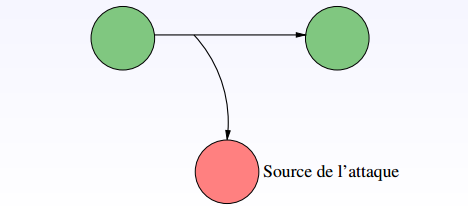
\includegraphics[width=\columnwidth]{img/but_intercep.png}
				\label{fig:but_intercep}
			\end{center}
		\end{figure}
		\newpage
		\textbf{Modification :} vise l'intégrité des informations (modification, rejeu, ...).
		
		\begin{figure}[!hbt]
			\begin{center}
				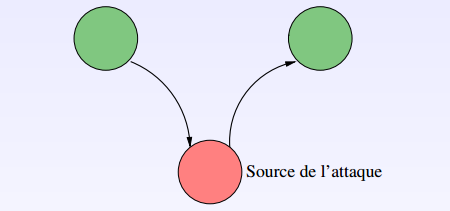
\includegraphics[width=\columnwidth]{img/but_modif.png}
				\label{fig:but_modif}
			\end{center}
		\end{figure}
		\textbf{Fabrication :} vise l'authenticité des informations (mascarade, ...).
		
		\begin{figure}[!hbt]
			\begin{center}
				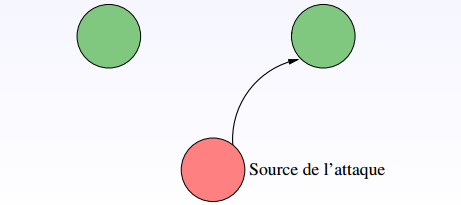
\includegraphics[width=\columnwidth]{img/but_fab.png}
				\label{fig:but_fab}
			\end{center}
		\end{figure}
		
	\subsection{Technique de recherche d'information}
		\begin{itemize}
			\item Recherche d'informations publiques : DNS, \verb|whois|, ...
			\item Découverte du réseau et du filtrage IP : \verb|traceroute|, \verb|ping|, \verb|hping|, \verb|netcat|, ...
			\item Découverte des systèmes d'exploitation : \verb|nessus|, \verb|nmap|, \verb|xprobe|, \verb|queso|, ...
			\item Découverte de services ouverts : \verb|nmap|, \verb|udp-scan|, \verb|nessus|, ...
			\item Découverte des versions logicielles : \verb|telnet|, \verb|netcat|, ...
		\end{itemize}
		
	\subsection{Exemple : découverte des machines via DNS}
		Interrogation du DNS avec \verb$dig$ :
		\begin{itemize}
			\item serveur de mail (champ MX), serveur DNS (champ NS)
			\item résolution inverse sur toutes les adresses (\textsl{peu discret}) : \verb$dig -x$
			\item transfert de zone (\textsl{pas toujours autorisé}) : \verb$dig server axfr zone.$
		\end{itemize}
		\begin{Verbatim}[fontsize=\small]
>dig labri.fr. MX
; <<>> DiG 9.4.1-P1 <<>> labri.fr. MX
;; global options: printcmd
;; Got answer:
;; ->>HEADER<<- opcode: QUERY, status:
NOERROR, id: 22464
...
;; QUESTION SECTION:
;labri.fr. IN MX
;; ANSWER SECTION:
labri.fr. 28800 IN MX 10 iona.labri.fr.
...
		\end{Verbatim}
		
	\subsection{Balayage}
	
		\subsubsection{Découverte de machines}
		~\\
			\textbf{But} : découvrir les machines d'un réseau donné.\\
			\textbf{Principe} : envoyer un paquet à toutes les adresses et analyser le paquet retour.\\
			\textbf{Outils} : \verb$nmap$.
		~\\
		\subsubsection{Découverte de ports ouverts}
		~\\
			\textbf{But} : découvrir les services/ports ouverts sur une machine donnée.\\
			\textbf{Principe} : envoyer des paquets et analyser les paquet retour (ou leur absence).\\
			\textbf{Outils} : \verb$nmap$, \verb$telnet$, \verb$netcat$, ...
		~\\
		\subsubsection{Techniques de balayage avec nmap}
		~\\
			\textit{ping sweep} (balayage avec ping) : \verb$nmap -sP -PI ...$\\
			\textbf{Principe} : envoyer un paquet \verb$ICMP Echo Request$ et attendre le paquet \verb$ICMP Echo Reply$.\\
			\textbf{Inconvénient} : méthode très peu discrète.\\
			~\\
			\textit{Techniques plus sophistiquées} : nécessite généralement des privilèges administrateur sur la machine source :
			\begin{itemize}
				\item \textit{Half Open SYN scan} (un seul paquet SYN)
				\item \textit{NULL scan} (paquet sans flags) (réponse uniqueent si le port correspondant est fermé)
				\item \textit{FIN scan} (un seul paquet avec le flag FIN)
				\item \textit{XMAS scan} (URG + PUSH + FIN)
				\item ...
			\end{itemize}
		~\\
		\subsubsection{Détection de ports ouverts}
		~\\
			\textbf{scan TCP via HTTP \textit{proxy bounce scan}} : utiliser un proxy HTTP comme relai pour faire du scan de ports :
			\begin{itemize}
				\item \verb$GET http://ftp.ens-lyon.fr:21 HTTP/1.0$ et attendre la réponse
			\end{itemize}
			\textbf{scan TCP via FTP \textit{FTP Bounce attack}} : utiliser un proxy FTP (ayant un disfonctionnement) comme relai pour faire du scan de ports :
			\begin{itemize}
				\item \verb$PORT 10,10,0,2,0,25$
				\item \verb$nmap -b ...$
			\end{itemize}
			\textbf{scan UDP} : \verb$nmap -sU ...$\\
			\textbf{scan RPC} : \verb$nmap -sR ...$
		
	\subsection{Détermination du filtrage IP}
	
		\textbf{Méthode} :
		\begin{itemize}
			\item forger un paquet avec un \textit{ttl} tel que le paquet soit arrêté par un filtre IP.
			\item Essayer d ecommuniquer avc un hôte situé derrière le firewall.
			\item Analyser les réponses.
		\end{itemize}
		\textbf{Outils} : firewalk, ...\\
		\textbf{Défense} : Interdir aux réponses ICMP de sortir du réseau protégé, \textbf{etc}.
	
	\subsection{Prise de contrôle d'un serveur distant}
		
		En plusieurs étapes :
		\begin{enumerate}
			\item Recherche de services ouverts (SMTP, FTP, ...)
			\item Exploitation de vulnérabilités : (CGI, exploit connu, débordement de buffer, injection de code/commande, ...)
			\item Pose de sniffer
			\item Pose de backdoor
		\end{enumerate}
		~\\
		Exemples de backdoor :\\
		\textbf{rwwwshell} : lancer un client HTTP avec un shell associé sur une machine à l'intérieur du réseau et ouvrir une connexion HTTP vers un serveur du pirate.\\
		\textbf{loki} : installer un serveur particulier sur une machine du réseau interne et communiquer avec lui en utilisant le champ données des paquets ICMP.
		
	\subsection{Attaques sur les réseaux locaux}
		
		\textbf{Ecoute du réseau : }capturer le contenu des paquets qui ne nous sont pas destinés :
		\begin{itemize}
			\item tcpdump
			\item sniff
			\item ...
		\end{itemize}

		\textbf{Usurpation d'adresses (IP et MAC) : }Forger et envoyer des paquets avec une fausse @IP :
		\begin{itemize}
			\item dsniff
			\item ...
		\end{itemize}

		\textbf{Vol de session : }Forger des paquets permettant la prise de contrôle d’une connexion déjà établie :
		\begin{itemize}
			\item juggernaut
			\item hunt
			\item ...
		\end{itemize}

	\subsection{Usurpation d'adresses (Spoofing)}

		Le principe est de forger et envoyer des paquets IP avec une fausse adresse source. Il est donc impossible de trouver la véritable source.\\
		C'est une technique souvent utilisée dans le cas d'attaque de type DoS\footnote{Une attaque de type DoS vise l'interruption d'un service en saturant la cible de requêtes}.

	\subsection{Vol de session (Connection Hijacking)}

		L'objectif est de prendre la main sur une connexion déjà établie.\\
		\textbf{Principe : }
		\begin{itemize}
			\item Attendre l'établissement d'une connexion
			\item Désynchroniser la connexion entre le client et le serveur (en forgeant un paquet avec un numéro de séquence particulier)
			\item Profiter de la désynchronisation pour faire faire au serveur ce que l'on veut
		\end{itemize}
		C'est une attaques très compliquée, voir impossible si l'on a pas la possibilité de voir le trafic entre le client et le serveur.

\section{Quelques cas concrets}

	\subsection{DNS : failles et dangers}
		
		\textbf{Présentation de DNS}\\
		C'est un protocole proposé en 1983, qui n'a pas beaucoup évolué depuis.\\
		C'est un mécanisme rapide et précis qui réalise la correspondance nom/@IP. DNS peut servir à plus que simplement renvoyer l'@IP d'un nom de domaine.\\
		DNS est le deuxième plus ancien protocole \textit{incontesté} dans ce qu'il fait\footnote{telnet a évolué vers ssh, FTP a été délaissé pour HTTP, ...}, il ne reste que SMTP qui est dans le même cas. Il est donc universellement utilisé et largement déployé.
		
		\textbf{Fonctionnement}\\
		On distingue deux types de fonctionnement lors d'une requête DNS :
		\begin{itemize}
			\item Récursif : si le serveur interrogé ne connaît pas la réponse, il va lui-même lancer une requête vers un autre serveur pour obtenir la réponse, qu'il garde en cache (au maximum 1 semaine en moyenne)
			\item Itératif : si le serveur interrogé ne connaît pas la réponse, il va simplement indiquer quel serveur interroger au client
		\end{itemize}
		
		La grosse faille des serveurs DNS est le fait qu'ils utilisent majoritairement le même port (53), et qu'il devient donc facile de spammer le cache d'un serveur. Ceci peut par contre avoir des effets collatéraux\footnote{casser la hiérarchie DNS et donc faire tomber internet}.
		
		Afin de patcher ce problème, il faudrait améliorer la randomisatin de numéro de requête (pour éviter le spamming), utiliser un port source aléatoire et à plus long terme, utiliser un protocole à signature électronique tel que DNSSec.
		
	\subsection{Honeypot}
	
		Le \textit{honeypot} est une technique qui laisse volontairement une machine ou plus souvent une partie du réseau (complètement séparé du reste) afin que les attaquants ciblent plus ce dernier. Un honeypot à deux principaux buts :
		\begin{itemize}
			\item Augmenter la sécurité du réseau
			\item Récupérer des informations sur les méthodes des attaquants
		\end{itemize}
		
		Cependant, cette méthode est assez visible car un honeypot laisse une empreinte qui peut être repérée.
		
\section{IPSec}

	Le besoin de sécurité s'est fait ressentir vers 1994\footnote{RFC 1636} avec la recrudescence des attaques de type spoofing.
	IPSec apporte plusieurs applications :
	\begin{itemize}
		\item Sécuriser une connexion de succursale sur internet
		\item Accès distant sécurisé sur internet
		\item Authenticité des paquets reçus
	\end{itemize}
	De plus, IPSec a les avantages d'être utilisé uniquement sur des communications spécifiques\footnote{sans perturber les autres communications}, d'être au dessous de la couche de transport (TCP, UDP) ce qui lui permet d'être transparent aux applications, ainsi qu'aux utilisateurs\footnote{une fois mis en place}.
	\begin{figure}[hbt!]
			\begin{tabular}{c|ccc}
				~ & AH & ESP (chi) & ESP (chif. + auth.) \\
				\hline
				Ctrl d'accès & X & X & X \\
				Intégr. hors co. & X & & X \\
				Auth. origine datas & X & & X \\
				Rejet paquets rejoués & X & X & X \\
				Confidentialité & & X & X \\
				Confi. flot trafic & & X & X \\
			\end{tabular}
			\caption{Services d'IPSec}
			\label{fig:ipsec_services}
	\end{figure}
		
	Une association de sécurité\footnote{AS} est une relation en sens unique entre un émetteur et un destinataire qui garantit les services de sécurité pour le trafic généré.\\
	Des services de sécurité sont alloués à une AS pour utiliser AH ou ESP, mais pas les deux.\\
	Une AS est définie par 3 paramètres :
	\begin{itemize}
		\item Index de paramètre de sécurité (IPS) : une chaîne binare assignée à cette AS et ayant une signification locale
		\item @IP de destination
		\item Identification du protocole de sécurité : indique si l'association est AH ou ESP
	\end{itemize}
	
	Plusieurs AS peuvent être combinées.\\
	Les associations entre AS et type de trafic se font pas le biais d'une base de données de politique de sécurité (SPD\footnote{Security Policy Database}).
	
	Il y a deux modes d'utilisation d'IPSec :
	\begin{itemize}
		\item Mode transport : sécurité au niveau de la couche transport, ESP chiffre (et optionnellement authentifie) uniquement l'information utile du paquet, AH authentifie l'information utile IP et des parties de l'en-tête
		\item Mode tunnel : sécurité du paquet tout entier, après l'ajout des champs AH ou ESP, le paquet entier est traité comme l'information utile du paquet IP externe. Au moins une extrémité de l'AS doit être une passerelle de sécurité\footnote{firewall, passerelle inplémentant IPSec, ...}
	\end{itemize}

	
% Your document ends here!
\end{document}